% Options for packages loaded elsewhere
\PassOptionsToPackage{unicode}{hyperref}
\PassOptionsToPackage{hyphens}{url}
%
\documentclass[
]{article}
\usepackage{amsmath,amssymb}
\usepackage{iftex}
\ifPDFTeX
  \usepackage[T1]{fontenc}
  \usepackage[utf8]{inputenc}
  \usepackage{textcomp} % provide euro and other symbols
\else % if luatex or xetex
  \usepackage{unicode-math} % this also loads fontspec
  \defaultfontfeatures{Scale=MatchLowercase}
  \defaultfontfeatures[\rmfamily]{Ligatures=TeX,Scale=1}
\fi
\usepackage{lmodern}
\ifPDFTeX\else
  % xetex/luatex font selection
\fi
% Use upquote if available, for straight quotes in verbatim environments
\IfFileExists{upquote.sty}{\usepackage{upquote}}{}
\IfFileExists{microtype.sty}{% use microtype if available
  \usepackage[]{microtype}
  \UseMicrotypeSet[protrusion]{basicmath} % disable protrusion for tt fonts
}{}
\makeatletter
\@ifundefined{KOMAClassName}{% if non-KOMA class
  \IfFileExists{parskip.sty}{%
    \usepackage{parskip}
  }{% else
    \setlength{\parindent}{0pt}
    \setlength{\parskip}{6pt plus 2pt minus 1pt}}
}{% if KOMA class
  \KOMAoptions{parskip=half}}
\makeatother
\usepackage{xcolor}
\usepackage[margin=1in]{geometry}
\usepackage{color}
\usepackage{fancyvrb}
\newcommand{\VerbBar}{|}
\newcommand{\VERB}{\Verb[commandchars=\\\{\}]}
\DefineVerbatimEnvironment{Highlighting}{Verbatim}{commandchars=\\\{\}}
% Add ',fontsize=\small' for more characters per line
\usepackage{framed}
\definecolor{shadecolor}{RGB}{248,248,248}
\newenvironment{Shaded}{\begin{snugshade}}{\end{snugshade}}
\newcommand{\AlertTok}[1]{\textcolor[rgb]{0.94,0.16,0.16}{#1}}
\newcommand{\AnnotationTok}[1]{\textcolor[rgb]{0.56,0.35,0.01}{\textbf{\textit{#1}}}}
\newcommand{\AttributeTok}[1]{\textcolor[rgb]{0.13,0.29,0.53}{#1}}
\newcommand{\BaseNTok}[1]{\textcolor[rgb]{0.00,0.00,0.81}{#1}}
\newcommand{\BuiltInTok}[1]{#1}
\newcommand{\CharTok}[1]{\textcolor[rgb]{0.31,0.60,0.02}{#1}}
\newcommand{\CommentTok}[1]{\textcolor[rgb]{0.56,0.35,0.01}{\textit{#1}}}
\newcommand{\CommentVarTok}[1]{\textcolor[rgb]{0.56,0.35,0.01}{\textbf{\textit{#1}}}}
\newcommand{\ConstantTok}[1]{\textcolor[rgb]{0.56,0.35,0.01}{#1}}
\newcommand{\ControlFlowTok}[1]{\textcolor[rgb]{0.13,0.29,0.53}{\textbf{#1}}}
\newcommand{\DataTypeTok}[1]{\textcolor[rgb]{0.13,0.29,0.53}{#1}}
\newcommand{\DecValTok}[1]{\textcolor[rgb]{0.00,0.00,0.81}{#1}}
\newcommand{\DocumentationTok}[1]{\textcolor[rgb]{0.56,0.35,0.01}{\textbf{\textit{#1}}}}
\newcommand{\ErrorTok}[1]{\textcolor[rgb]{0.64,0.00,0.00}{\textbf{#1}}}
\newcommand{\ExtensionTok}[1]{#1}
\newcommand{\FloatTok}[1]{\textcolor[rgb]{0.00,0.00,0.81}{#1}}
\newcommand{\FunctionTok}[1]{\textcolor[rgb]{0.13,0.29,0.53}{\textbf{#1}}}
\newcommand{\ImportTok}[1]{#1}
\newcommand{\InformationTok}[1]{\textcolor[rgb]{0.56,0.35,0.01}{\textbf{\textit{#1}}}}
\newcommand{\KeywordTok}[1]{\textcolor[rgb]{0.13,0.29,0.53}{\textbf{#1}}}
\newcommand{\NormalTok}[1]{#1}
\newcommand{\OperatorTok}[1]{\textcolor[rgb]{0.81,0.36,0.00}{\textbf{#1}}}
\newcommand{\OtherTok}[1]{\textcolor[rgb]{0.56,0.35,0.01}{#1}}
\newcommand{\PreprocessorTok}[1]{\textcolor[rgb]{0.56,0.35,0.01}{\textit{#1}}}
\newcommand{\RegionMarkerTok}[1]{#1}
\newcommand{\SpecialCharTok}[1]{\textcolor[rgb]{0.81,0.36,0.00}{\textbf{#1}}}
\newcommand{\SpecialStringTok}[1]{\textcolor[rgb]{0.31,0.60,0.02}{#1}}
\newcommand{\StringTok}[1]{\textcolor[rgb]{0.31,0.60,0.02}{#1}}
\newcommand{\VariableTok}[1]{\textcolor[rgb]{0.00,0.00,0.00}{#1}}
\newcommand{\VerbatimStringTok}[1]{\textcolor[rgb]{0.31,0.60,0.02}{#1}}
\newcommand{\WarningTok}[1]{\textcolor[rgb]{0.56,0.35,0.01}{\textbf{\textit{#1}}}}
\usepackage{graphicx}
\makeatletter
\def\maxwidth{\ifdim\Gin@nat@width>\linewidth\linewidth\else\Gin@nat@width\fi}
\def\maxheight{\ifdim\Gin@nat@height>\textheight\textheight\else\Gin@nat@height\fi}
\makeatother
% Scale images if necessary, so that they will not overflow the page
% margins by default, and it is still possible to overwrite the defaults
% using explicit options in \includegraphics[width, height, ...]{}
\setkeys{Gin}{width=\maxwidth,height=\maxheight,keepaspectratio}
% Set default figure placement to htbp
\makeatletter
\def\fps@figure{htbp}
\makeatother
\setlength{\emergencystretch}{3em} % prevent overfull lines
\providecommand{\tightlist}{%
  \setlength{\itemsep}{0pt}\setlength{\parskip}{0pt}}
\setcounter{secnumdepth}{-\maxdimen} % remove section numbering
\ifLuaTeX
  \usepackage{selnolig}  % disable illegal ligatures
\fi
\IfFileExists{bookmark.sty}{\usepackage{bookmark}}{\usepackage{hyperref}}
\IfFileExists{xurl.sty}{\usepackage{xurl}}{} % add URL line breaks if available
\urlstyle{same}
\hypersetup{
  pdftitle={Práctica dirigida 10},
  hidelinks,
  pdfcreator={LaTeX via pandoc}}

\title{Práctica dirigida 10}
\author{}
\date{\vspace{-2.5em}}

\begin{document}
\maketitle

{
\setcounter{tocdepth}{1}
\tableofcontents
}

\includegraphics[width=0.3\linewidth]{logoPUCP}

\hypertarget{i.-anuxe1lisis-de-regresiuxf3n-simple-ideas-clave}{%
\section{\texorpdfstring{\textbf{I. Análisis de regresión simple: ideas
clave}}{I. Análisis de regresión simple: ideas clave}}\label{i.-anuxe1lisis-de-regresiuxf3n-simple-ideas-clave}}

Técnica estadística que predice el valor de una variable con los valores
de otra. La regresión lineal simple es un método útil para predecir una
respuesta cuantitativa \textbf{Y} partiendo de una sola variable
predictora \textbf{X}, asumiendo que hay una relación aproximadamente
lineal entre X e Y. Matemáticamente, esta relación lineal se representa
como

Y = a + bX + E

\begin{itemize}
\item
  Y = variable dependiente o explicada. Variable cuyos valores se desea
  predecir o resumir. Un modelo de regresión lineal tiene como variable
  dependiente una variable numérica
\item
  a = Constante: ordenada en el origen, valor esperado de ``Y'' cuando
  X=0
\item
  b = Pendiente: mide el cambio de la variable ``Y'' por cada unidad de
  cambio de ``X''. Su magnitud sirve para predecir en cuánto aumentará
  ``y'' cada vez que ``x'' se incremente en una unidad.Su signo puede
  ser positivo o negativo, y en esto la interpretación coincide con la
  correlación.
\item
  X = variable utilizada para predecir el valor de la variable
  dependiente. También se denomina variable predictora o variable
  explicativa. Las variables explicativas que son parte del modelo
  suelen ser numéricas o intervalares; sin embargo, es posible
  incorporar variables explicativas ordinales o categóricas.
\item
  E = Corresponde a las desviaciones de los valores verdaderos de Y con
  respecto a los valores esperados de ``Y'' (diferencia entre lo
  observado y estimado por el modelo). Asumimos que es independiente de
  ``X''.
\end{itemize}

La relación entre las variables depende de la pendiente:

\begin{itemize}
\item
  Si b es positivo, Y aumenta cuando X aumenta. Es una relación directa
  / positiva.
\item
  Si b es negativo, Y aumenta cuando X disminuye. Es una relación
  inversa / negativa.
\item
  Si b es cero.Y no cambia cuando X varía. No existe relación entre las
  variables.
\end{itemize}

Asimismo, con el método de la regresión lineal se puede responder las
siguientes preguntas:

\begin{itemize}
\item
  Analizar si hay una \textbf{asociación} entre las variables mediante
  un test de independencia estadística.
\item
  Analizar la \textbf{dirección} de la asociación (directa o inversa).
\item
  Evaluar la \textbf{fuerza} de la asociación usando una medida de
  asociación llamada \emph{correlación de Pearson}.
\item
  Estimar una ecuación de regresión que \textbf{``predice''} los valores
  de la variable dependiente para valores de la variable independiente.
\end{itemize}

\hypertarget{ii.-aplicaciuxf3n-pruxe1ctica}{%
\section{\texorpdfstring{\textbf{II. Aplicación
práctica}}{II. Aplicación práctica}}\label{ii.-aplicaciuxf3n-pruxe1ctica}}

Para la sesión de hoy trabajaremos con datos del 2017 de una base de
datos que contiene variables obtenidas de las siguientes bases: -
Freedom in the World - V-Dem - Democracy Index - Global Corruption
Barometer

Información sobre las bases: - Freedom in the World es elaborado por
Freedom House y analiza los siguientes aspectos: el proceso electoral,
las políticas pluriculturales y la participación, el funcionamiento del
gobierno, la libertad de expresión y de creencia, los derechos de
asociación y organización, el estado de derecho, la autonomía personal y
los derechos individuales.

\begin{itemize}
\item
  V-Dem es publicada por el V-Dem Institute. En ella se describe la
  calidad de los gobiernos a partir de información de 542 indicadores.
  La sata describe todos los aspectos de un gobierno, brindándo énfasis
  en la calidad de la democracia, la inclusividad y otros indicadores
  económicos.
\item
  Democracy Index es elaborado por The Economist y utiliza 60
  indicadores, agrupados en cinco categorías: proceso electoral y
  pluralismo, libertades civiles, funcionamiento del gobierno,
  participación política y política cultural. A partir de estas
  categorías posiciona a los países en alguno de los cuatro tipos de
  régimen: Democracia plena, democracia imperfecta, régimen híbrido y
  régimen autoritario.
\item
  Global Corruption Barometer es publicado por Transparencia
  Internacional y contiene información proveniente de la opinión pública
  ciudadana
\end{itemize}

\begin{Shaded}
\begin{Highlighting}[]
\FunctionTok{library}\NormalTok{(rio)}
\NormalTok{data}\OtherTok{=}\FunctionTok{import}\NormalTok{(}\StringTok{"corrupcion{-}democracia{-}1.xlsx"}\NormalTok{)}
\end{Highlighting}
\end{Shaded}

Ejercicio 1: Impacto del índice de democracia participativa en \% de
personas que personas que opinan que la mayoría de autoridades están
implicada en corrupción por país

Las variables que utilizaremos serán:

\textbf{Q2c} = Porcentaje de personas que opinan que la mayoría o todos
los funcionarios del gobierno están envueltos en corrupción

\textbf{Part} = Indicador de democracia participativa - Vdem

\hypertarget{gruxe1fico-de-dispersiuxf3n}{%
\subsection{Gráfico de dispersión:}\label{gruxe1fico-de-dispersiuxf3n}}

\textbf{¿El indicador de democracia participativa tiene un impacto en el
porcentaje de personas que opinan que la mayoría/todos los funcionarios
están envueltos en corrupción?}

Elaboramos el gráfico de dispersión y la recta

\begin{Shaded}
\begin{Highlighting}[]
\FunctionTok{library}\NormalTok{(dplyr)}
\FunctionTok{library}\NormalTok{(ggplot2)}
\NormalTok{data }\SpecialCharTok{\%\textgreater{}\%}
  \FunctionTok{ggplot}\NormalTok{(}\FunctionTok{aes}\NormalTok{ (}\AttributeTok{x=}\NormalTok{Q2c}\SpecialCharTok{*}\DecValTok{100}\NormalTok{, }\AttributeTok{y=}\NormalTok{Part)) }\SpecialCharTok{+}
  \FunctionTok{geom\_point}\NormalTok{(}\AttributeTok{colour=}\StringTok{"lightsteelblue4"}\NormalTok{) }\SpecialCharTok{+}  
  \FunctionTok{xlab}\NormalTok{(}\StringTok{"\% de personas que opinan }\SpecialCharTok{\textbackslash{}n}\StringTok{ que la mayoría/todos  los funcionarios }\SpecialCharTok{\textbackslash{}n}\StringTok{ }
\StringTok{       públicos están involucrados en corrupción"}\NormalTok{) }\SpecialCharTok{+}  
  \FunctionTok{ylab}\NormalTok{(}\StringTok{"Índicador de democracia participativa"}\NormalTok{)}\SpecialCharTok{+} \FunctionTok{theme\_light}\NormalTok{() }\SpecialCharTok{+} 
  \FunctionTok{geom\_smooth}\NormalTok{(}\AttributeTok{method=}\StringTok{"lm"}\NormalTok{, }\AttributeTok{se =}\NormalTok{ T, }\AttributeTok{colour=}\StringTok{"grey5"}\NormalTok{)}
\end{Highlighting}
\end{Shaded}

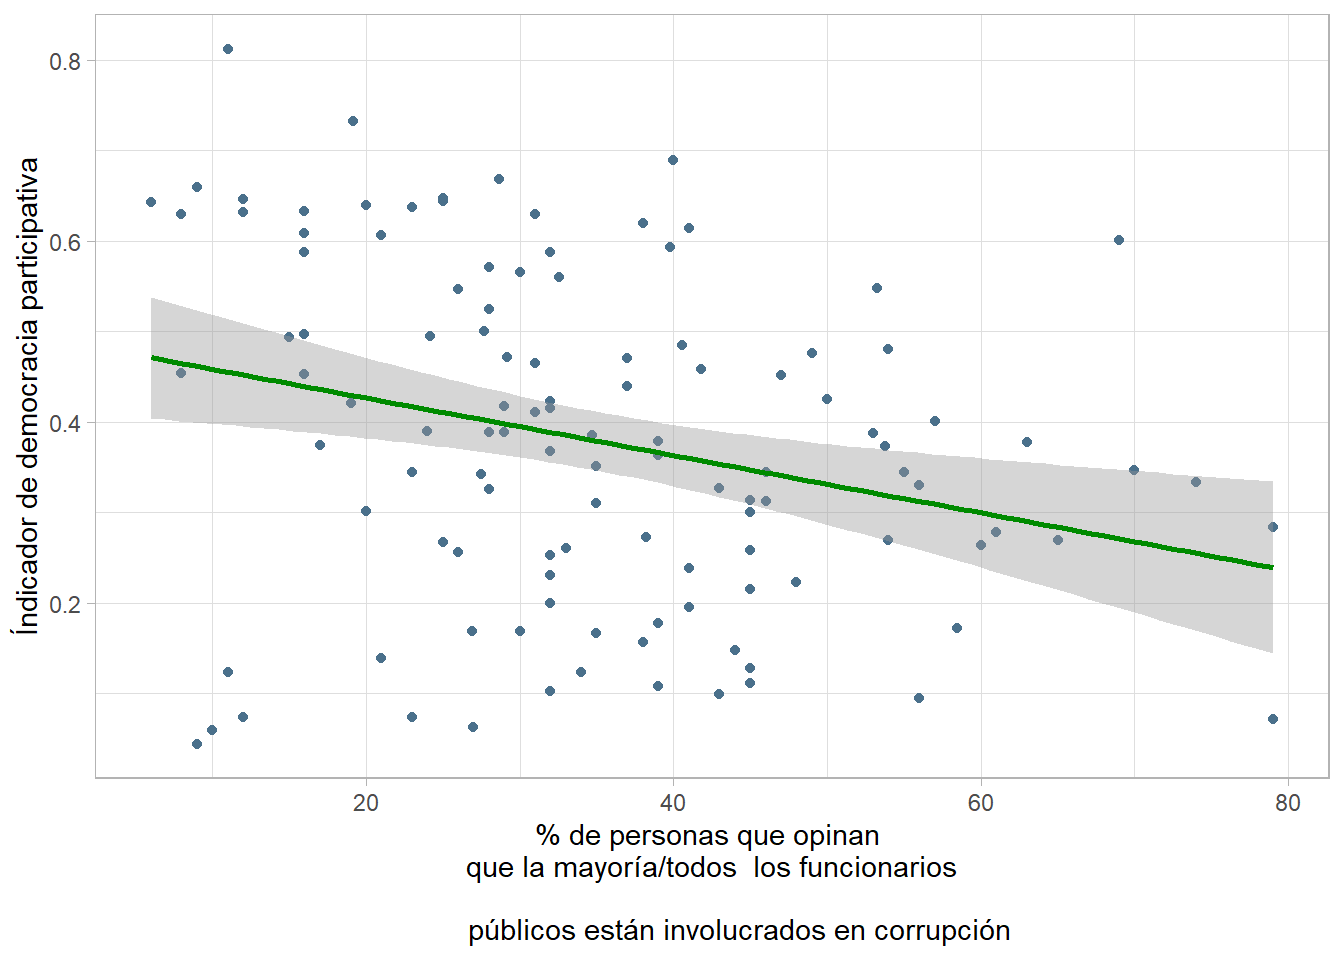
\includegraphics{pd10_files/figure-latex/unnamed-chunk-3-1.pdf}

A primera vista parece haber un leve impacto, y la relación entre
nuestras variables se perfila como negativa. Comprobémoslo \ldots{}

\hypertarget{creaciuxf3n-del-modelo}{%
\subsection{Creación del modelo}\label{creaciuxf3n-del-modelo}}

\begin{Shaded}
\begin{Highlighting}[]
\NormalTok{modelo1}\OtherTok{=}\FunctionTok{lm}\NormalTok{(Part}\SpecialCharTok{\textasciitilde{}}\NormalTok{Q2c,}\AttributeTok{data=}\NormalTok{data)}
\FunctionTok{summary}\NormalTok{(modelo1)}
\end{Highlighting}
\end{Shaded}

\begin{verbatim}
## 
## Call:
## lm(formula = Part ~ Q2c, data = data)
## 
## Residuals:
##      Min       1Q   Median       3Q      Max 
## -0.41744 -0.12712  0.00909  0.13936  0.35691 
## 
## Coefficients:
##             Estimate Std. Error t value Pr(>|t|)    
## (Intercept)  0.49004    0.03944  12.425  < 2e-16 ***
## Q2c         -0.31779    0.10258  -3.098  0.00245 ** 
## ---
## Signif. codes:  0 '***' 0.001 '**' 0.01 '*' 0.05 '.' 0.1 ' ' 1
## 
## Residual standard error: 0.1768 on 114 degrees of freedom
##   (2 observations deleted due to missingness)
## Multiple R-squared:  0.07765,    Adjusted R-squared:  0.06956 
## F-statistic: 9.598 on 1 and 114 DF,  p-value: 0.002453
\end{verbatim}

\hypertarget{interpretaciuxf3n}{%
\subsection{Interpretación}\label{interpretaciuxf3n}}

\emph{¿El porcentaje de personas que creen que los funcionarios son
corruptos influyen en el indicador de democracia participativa?}

Para interpretar los resultados del modelo debemos tener presente lo
siguiente:

\hypertarget{primero-p-value}{%
\subsubsection{Primero: p-value}\label{primero-p-value}}

Sabremos si la variable independiente impacta en la dependiente al
revisar la significancia del p valor.

Establezcamos nuestras hipótesis:

\begin{itemize}
\item
  H0: El modelo de regresión no es válido
\item
  H1: El modelo de regresión es válido (variable X aporta al modelo)
\end{itemize}

Como el p valor es \textbf{0.002453}, entonces podemos afirmar que hay
suficiente evidencia para rechazar la H0, por lo que concluimos que el
modelo sí es válido como modelo de predicción. Es decir, podemos decir
que hay evidencia estadística suficiente para afirmar que existe una
relación significativa entre el índice de democracia participativa y la
percepción de funcionarios corruptos por país.

En otras palabras, podemos decir que la percepción de funcionarios
corruptos del país \emph{sí influye} en el puntaje obtenido en el índice
de democracia participativa.

\hypertarget{segundo-pendienteb}{%
\subsubsection{Segundo: pendiente/b}\label{segundo-pendienteb}}

Explica cómo es el efecto de x en y. Para ello analizamos el valor del
parámetro de la pendiente.

En este caso, al ser este valor \textbf{-0.31779}, concluímos que cada
vez que el valor de la percepción de corrupción en el país aumenta en 1,
el puntaje del índice de democracia participativa disminuye en 0.318. Es
decir, tenemos una \emph{relación inversa o negativa}.

\hypertarget{tercero-r2}{%
\subsubsection{\texorpdfstring{Tercero:
R\textsuperscript{2}}{Tercero: R2}}\label{tercero-r2}}

Analizar cuánto de la variabilidad de la variable dependiente (y) es
explicada por la variable independiente (x), para ello revisamor el
\textbf{R\textsuperscript{2}} (Multiple R-squared). Los valores van de 0
a 1. Mientras más cercano esté el R2 a 1, mayor será la variabilidad
explicada. El R2 es un indicador de ajuste del modelo.

En nuestro modelo, este arrojó el valor de \textbf{0.07765}, por lo que
podemos concluir que aproximadamente el \textbf{7.8\%} (0.07765*100)de
la variabilidad en el índice de democracia participativa puede ser
explicado porel porcentaje de personas que opinan que la mayoría/todos
los funcionarios están envueltos en corrupción.

Esto quiere decir que la cantidad de variabilidad explicada es
relativamente baja. Por lo que podemos afirmar que hay otros factores
más importantes o complejos que afectan la percepción de corrupción en
cada país.

\hypertarget{cuarto-ecuaciuxf3n-de-la-recta}{%
\subsubsection{Cuarto: Ecuación de la
recta}\label{cuarto-ecuaciuxf3n-de-la-recta}}

Hallar la ecuación de la recta del modelo. Para lograrlo, revisemos los
dos valores de la tabla que se encuentran en la columna de ``Estimate'',
el valor de la primera fila es el del intercepto (a) y el de la segunda
es el de la pendiente (b).

Del segundo paso, ya conocíamos que el valor de la pendiente es
\textbf{-0.31779.} Si volvemos a revisar nuestra tabla podemos observar
que en el cruce de Estimate e Intercept está el valor de
\textbf{0.49004}, este sería nuestro intercepto. Ahora, armemos nuestra
ecuación de la recta:

\textbf{Ŷ = 0.49004 - 0.31779∗X}

Donde:

\begin{itemize}
\tightlist
\item
  X = Porcentaje de personas que opinan que la mayoría o todos los
  funcionarios del gobierno están envueltos en corrupción -
  (independiente)
\item
  Y = Indicador de democracia participativa - (dependiente)
\end{itemize}

\textbf{¿Qué se quiere saber?}: Queremos saber si el \% de personas que
opinan que los funcionarios son corruptos influye en el indicador de
democracia participativa.

Esa ecuación crea una línea recta en el diagrama de dispersión que
representa la relación entre ambas variables y además indica que el
cambio esperado en nuestra variable dependiente (Porcentaje de personas
que opinan que la mayoría o todos los funcionarios del gobierno están
envueltos en corrupción) por cada cambio de una unidad en nuestra
variable independiente (Indicador de democracia participativa). Así, con
esta ecuación se puede estimar el valor de Y para cualquier valor de X.

También podemos obtener los coeficientes de intercepción/intercepto y
pendiente de la siguiente forma:

\begin{Shaded}
\begin{Highlighting}[]
\NormalTok{modelo1}\SpecialCharTok{$}\NormalTok{coefficients}
\end{Highlighting}
\end{Shaded}

\begin{verbatim}
## (Intercept)         Q2c 
##   0.4900430  -0.3177901
\end{verbatim}

\hypertarget{quinto-predecir}{%
\subsubsection{Quinto: Predecir}\label{quinto-predecir}}

Podemos utilizar la relación linear establecida por la ecuación para
estimar el valor de la variable dependiente (Y) para un valor dado de la
variable independiente (X).

Por ejemplo, si queremos calcular el valor de porcentaje de personas que
opinan que la mayoría/todos los funcionarios están envueltos en
corrupción cuando el índice de democracia participativa (0 a 1) es 0.4,
solo tenemos que reemplazar el valor de x por 0.4 en nuestra ecuación.

Sustituyendo el valor de ``x'' en la ecuación, tenemos:

\textbf{Ŷ = 0.49004 - 0.31779 * 0.4}

\textbf{Ŷ = 0.49004 - 0.12712}

\textbf{Ŷ = 0.36292}

Por lo tanto, utilizando la ecuación de la recta, cuando el índice de
democracia participativa es 0.4 , podemos predecir que aproximadamente
el 36.2\% de las personas opinan que la mayoría/todos los funcionarios
están envueltos en corrupción en ese país.

Practica resolviendo los siguientes ejercicios

Ejercicio 2: Impacto de la puntuación de libertad en el \% de personas
que opinan que el nivel de corrupción disminuyó en el país

Ejercicio 3: Impacto del \% de personas que están de acuerdo con la
frase ``Denunciaría un caso de corrupción aunque tuviera que pasar un
día en el juzgado para declarar'' en el \% de personas que está de
acuerdo con que los ciudadanos de a pie creen que pueden hacer la
diferencia en la lucha contra la corrupción en el país

\end{document}
